% \documentclass{article}
% \usepackage[utf8]{inputenc}
% \usepackage[spanish]{babel}
% \usepackage{hyperref} % Allows hyperlinks
% 
% \usepackage[style=authoryear,sorting=nyt]{biblatex}
% \addbibresource{biblio.bib}
% \usepackage{csquotes} % 'babel/polyglossia' detected but 'csquotes' missing. Loading 'csquotes' recommended.
% 
% \title{Modelo lineal general}
% \author{Zeus Chiripa}
% \date{Octubre 2017}

% \begin{document}

% \maketitle

\section{Introducción}

El modelo lineal general (GLM, por sus siglas en inglés) es uno de los análisis estadísticos por excelencia en los datos obtenidos mediante técnicas de imagen cerebral. Los GLM son una herramienta estadística muy flexible y que pueden ser aplicados para evaluar métodos de efectos fijos como por ejemplo regresiones múltiples, análisis de varianza multivariante (MANOVA) o análisis de covarianza (MANCOVA). Además, y a pesar de su apelativo de lineal, este tipo de modelos pueden introducir elementos no lineales \cite{chung2013statistical}.

Los GLM permiten evaluar de una manera sencilla y eficaz relaciones entre variables a la vez que toma en cuenta el posible efecto de una covariable, es decir, una variable que no es de interés directo sobre el efecto a estudiar. Por ende, el GLM es una herramienta estadística muy completa para comprobar hipótesis entre variables. Por ejemplo, el GLM aplicado a los datos obtenidos mediante imágenes de resonancia magnética funcional (fMRI) permite ajustar con relativa sencillez otros modelos estadísticos como la función de la respuesta hemodinámica (HRF, por sus siglas en inglés) en un estudio relacionado a eventos o en un diseño por bloques \cite{lazar2008statistical}.

El GLM se define de la siguiente manera:

\begin{center}
  $Y = X\cdot\beta + \epsilon$
\end{center}

Donde $Y$ es la respuesta a modelar, $X$ es la matriz de variables predictoras, $\beta$ son los coeficientes asociados a cada una de las variables predictoras y $\epsilon$ representa al error, que por lo general se asume que tiene una distribución normal con media cero y varianza conocida ($\sigma^2$).

En fMRI, por lo general, $Y$ suele ser la matriz de datos, i.e., una matriz con el valor obtenido por cada voxel\footnote{\textit{Voxel}: es la unidad de información gráfica que define un punto dentro de un espacio tridimensional. En resonancia magnética corresponde a los puntos dentro del volumen que corresponde a la imagen.} a lo largo del tiempo (i.e., por cada tiempo de muestreo o \textit{time point} [Tp]); $X$ suele representar una matriz con los estímulos presentados a lo largo del tiempo, i.e., la matriz del diseño experimental. Por consiguiente, este modelo asume que los datos obtenidos por fMRI pueden explicarse por una combinación lineal de las variables del diseño experimental con un error estadísticamente normal asociado (que puede interpretarse como ruido gaussiano). En realidad, se trata de una asunción muy reduccionista para un fenómeno tan complejo como son los datos de fMRI, sin embargo, aquí radica una de las principales ventajas del GLM y es su simplicidad, dado que con un cálculo computacionalmente sencillo puede minimizar el error asociado al ajuste del modelo.

De la manera más simplificada, el GLM asume que cada voxel y cada Tp es independiente el uno del otro, y que la varianza del error ($\epsilon$) es constante a lo largo de todos los voxels. En este caso, la estimación de los coeficientes $\beta$ se puede obtener mediante mínimos cuadrados ordinarios.

Sin embargo, $X$ suele ir acompañada de varias covariables además de la distribución del diseño de bloques (e.g., variable binaria: ausencia o no del estímulo). Por lo general, se suele incorporar una predicción de la respuesta hemodinámica, mediante una convolución del diseño experimental con un modelo de HRF. Esta consideración emula el hecho de que la señal dependiente del nivel de oxigenación en sangre (o señal BOLD, por sus siglas en inglés, \cite{OgawaS1990}) no se hace patente inmediatamente tras la presencia del estímulo y que tiene un decaimiento antes de regresar al estado basal (ver más en detalle el Capítulo \ref{cap:origenBold}).

Además de esta implementación, el GLM es bastante flexible a la hora de incluir otras covariables como pueden ser las características específicas de un sujeto, al grupo al que pertenece (e.g., grupo experimental o grupo control), etc. Es decir, no solamente se restringe al análisis individual de un solo sujeto sino que puede generalizarse el mismo modelo para un grupo de sujetos e incluso para evaluar posibles diferencias entre los grupos.


\section{Modelaje de la señal de Resonancia Magnética funcional}

El análisis estadístico de la señal de fMRI es una de las últimas etapas en un estudio de resonancia magnética. Previamente la señal obtenida ha sido corregida y preprocesada (e.g., corrección de movimiento, filtrado, suavizado, normalización a un espacio estándar, etc.), por tanto, hay que tener en cuenta que se trata de una señal de unidades arbitrarias manipulada.

En la figura \ref{fig:glm01} podemos observar como la señal BOLD se ajusta bastante bien con los bloques de una tarea en particular. Sin embargo, como se comentó en el apartado anterior hay un cierto desfase de la señal sobre el bloque debido al comportamiento de la respuesta hemodinámica. Para limitar este efecto se suele aplicar una convolución de un modelo matemático de la HRF a la matriz del diseño ($X$).


\begin{figure}
	\begin{figg}
    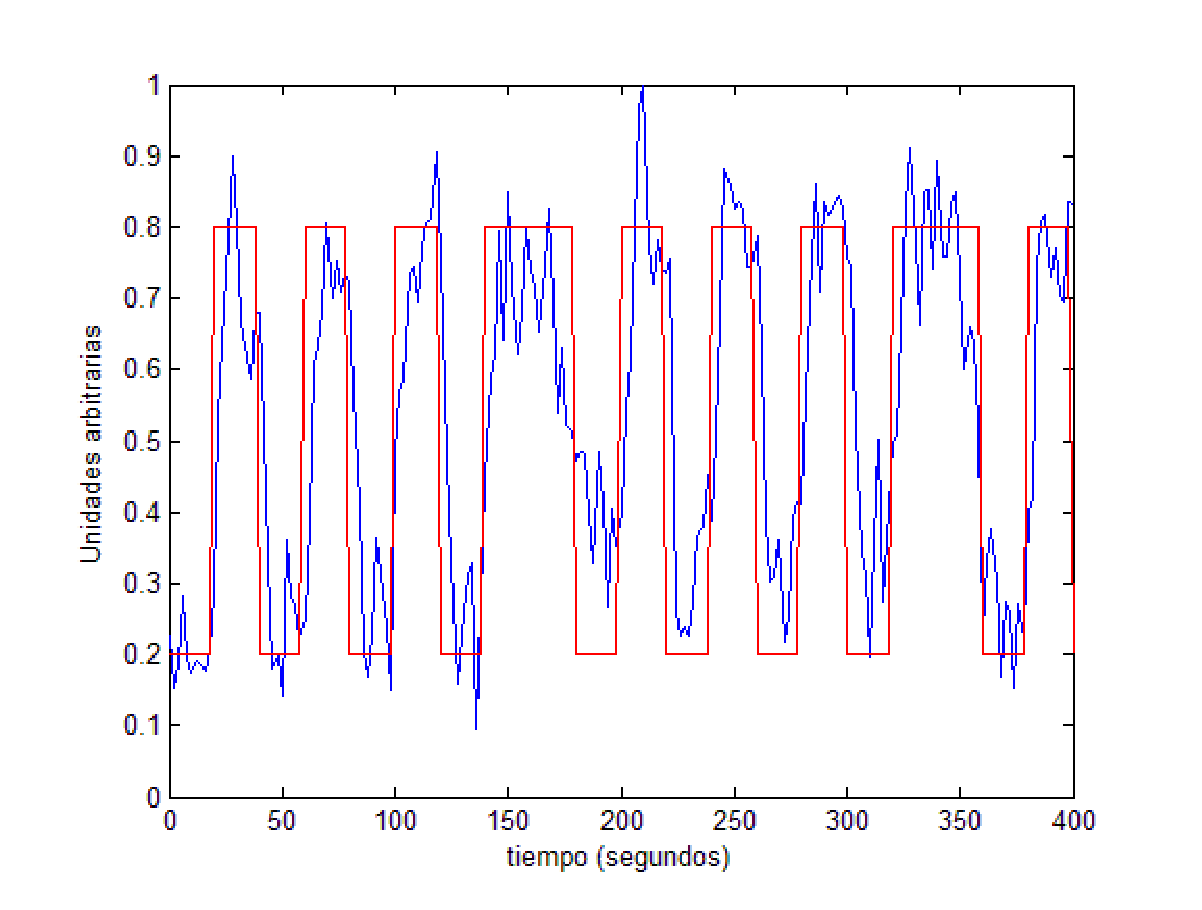
\includegraphics [width=0.7\textwidth]{glm_figura01.eps}
    \caption{Señal BOLD (azul) en un único \textit{voxel} a lo largo del tiempo en un estudio de fMRI bajo diseño de bloques (rojo).}
    \label{fig:glm01}
    \end{figg}
\end{figure}


La convolución se trata de una multiplicación aditiva de dos funciones. En este sentido, asumimos que la respuesta hemodinámica cerebral es un sistema que dado un estímulo su respuesta se puede modelar como la multiplicación aditiva lineal de la aparición o no aparición del estímulo (función 1) y un modelo canónico de dicha respuesta, i.e., la HRF (función 2).

En términos generales, podemos definir a un sistema como un proceso donde una señal de entrada es transformada en otra señal de salida. A modo de simplificación podemos asumir que el cerebro es un sistema que procesa las señales de entrada de un modo lineal respecto a las señales de salida. Es decir, podemos modelar el cerebro como un sistema lineal de tiempo invariante o sistema LTI, lo cual va a permitir trabajar de manera muy eficiente con las matrices del GLM \cite{cohen1997parametric}, dado que tiene las propiedades lineales de ser multiplicativo y aditivo, así como de independencia entre las respuestas \cite{vazquez1998nonlinear}.



\begin{figure}
	\begin{figg}
    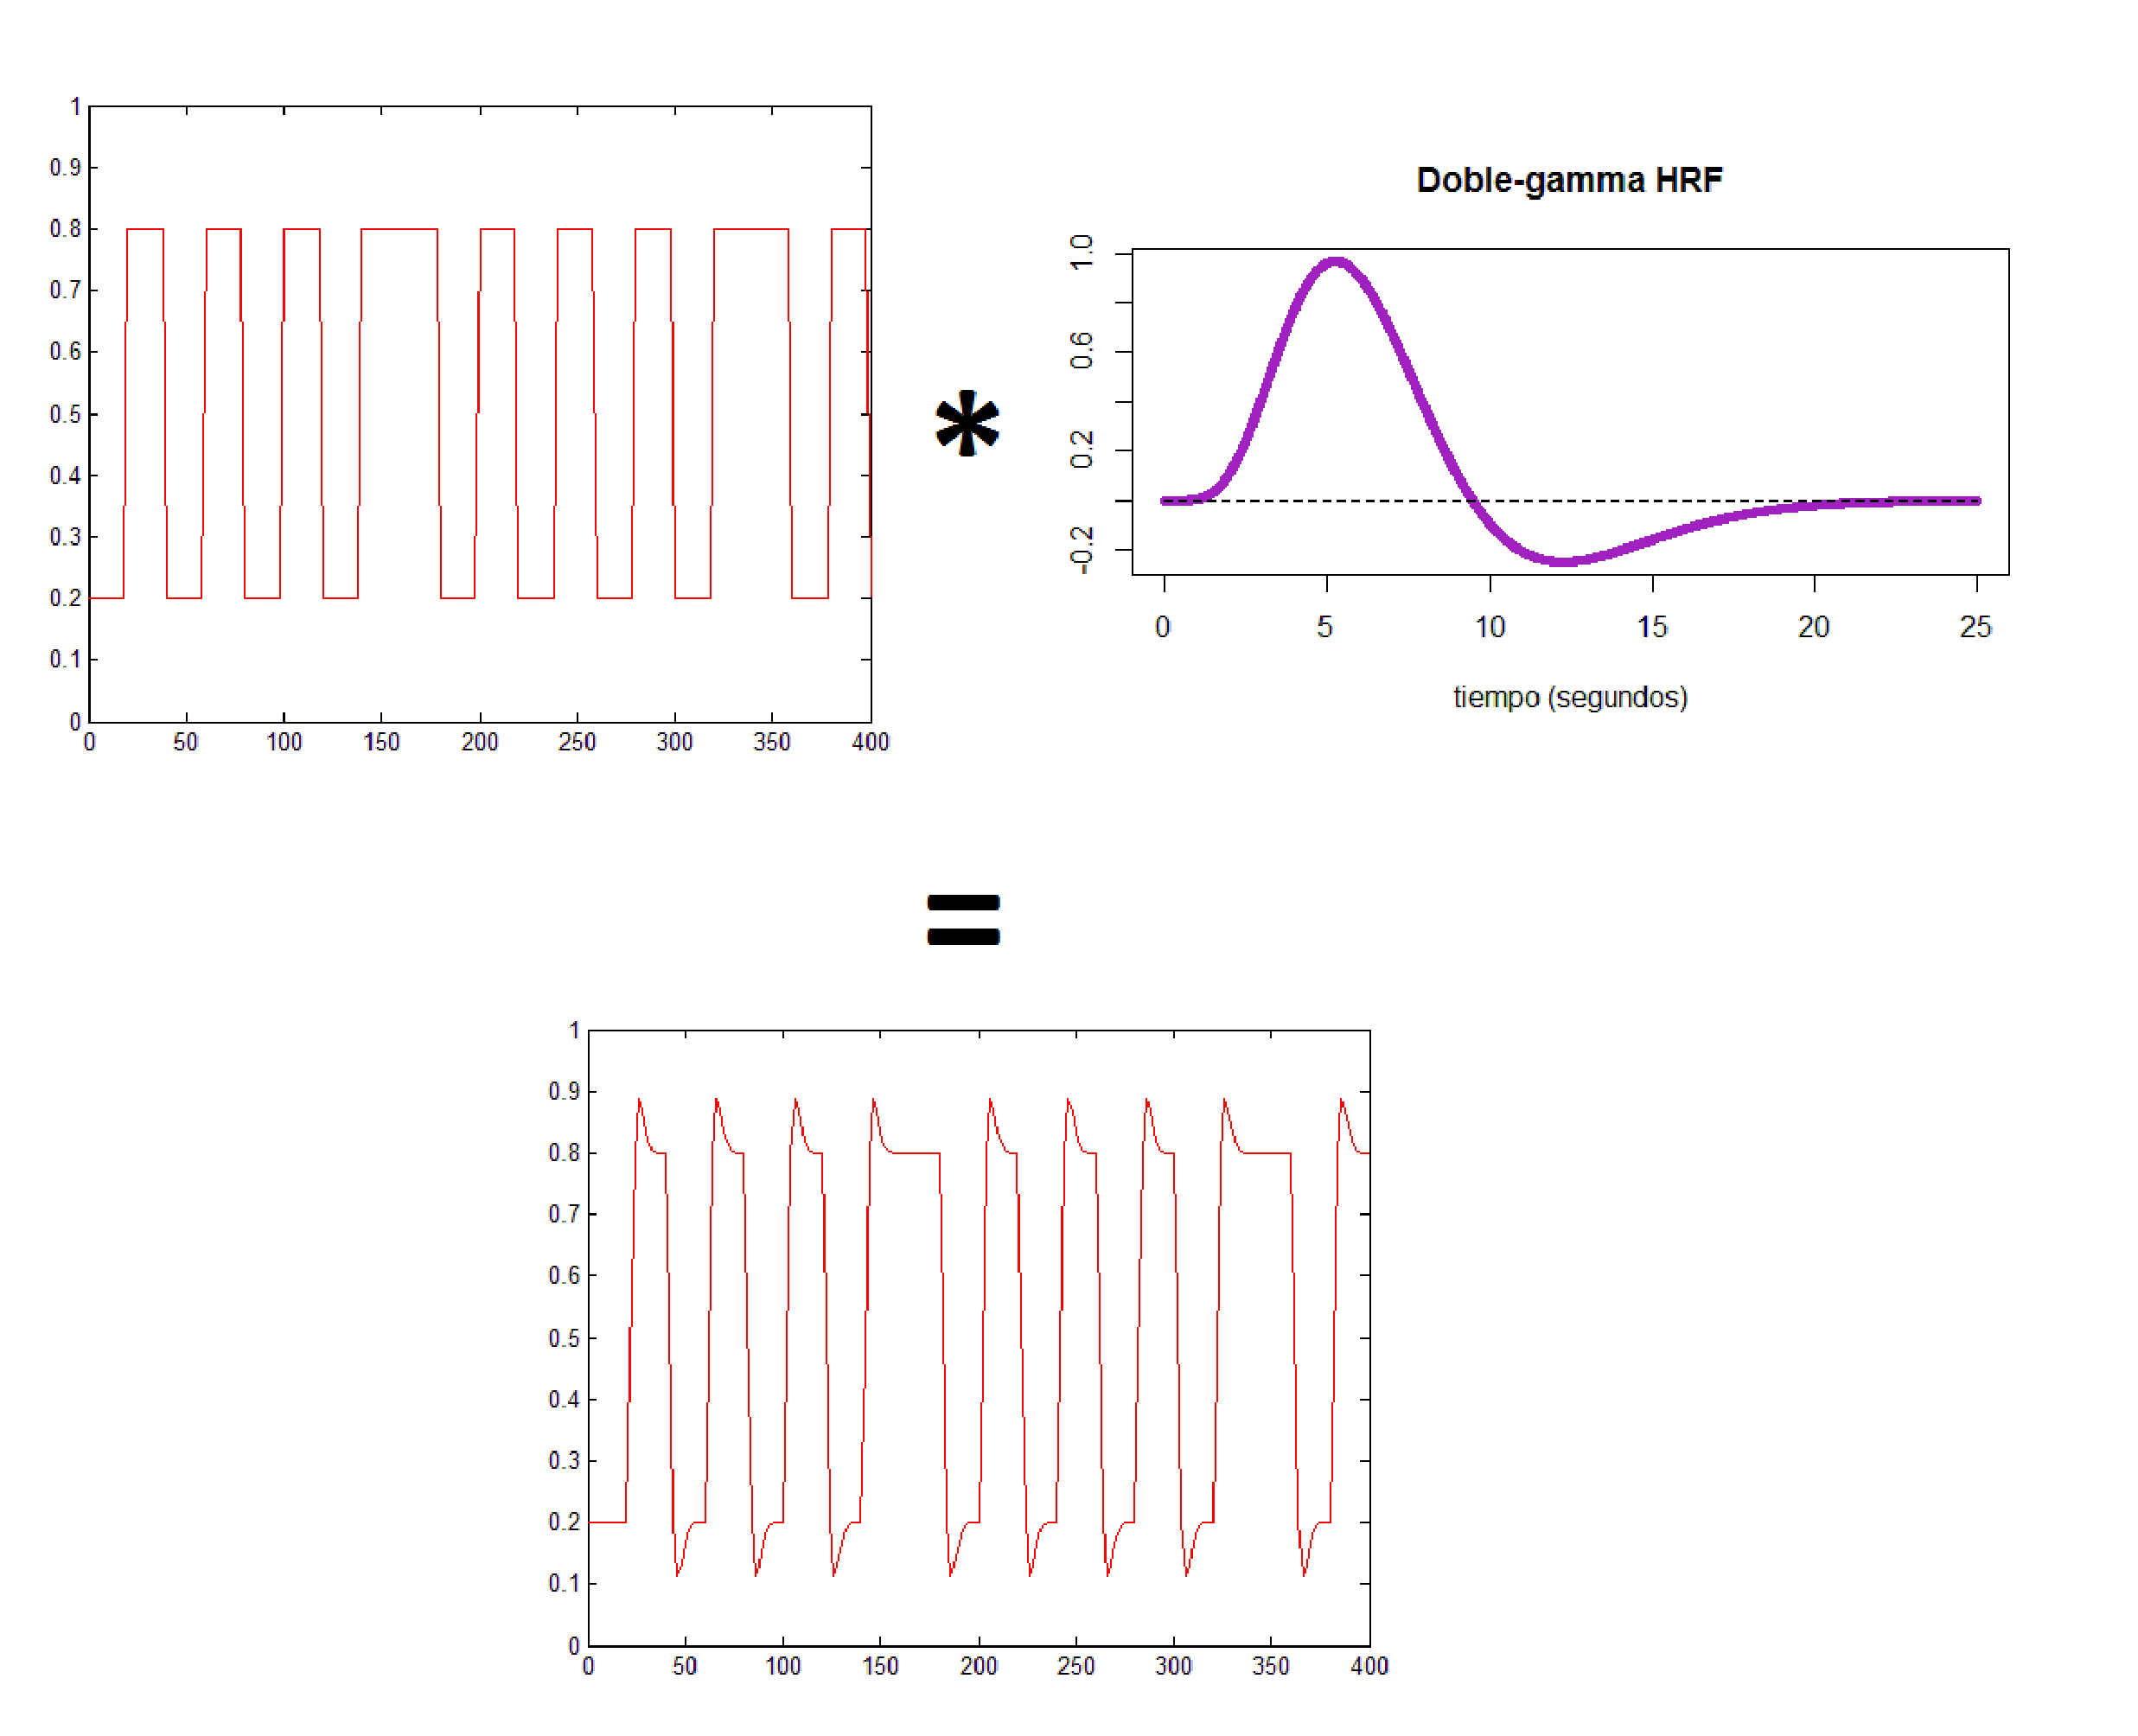
\includegraphics [width=0.7\textwidth]{glm_figura02.eps}
    \caption{Convolución (cuyo símbolo matemático es un asterisco) de un diseño de bloques con una HRF de doble gamma y su resultado consiguiente.}
    \label{fig:glm02}
    \end{figg}
\end{figure}

En la figura \ref{fig:glm02}, se ilustra un ejemplo de la señal predicha de una señal de entrada (diseño de bloques) que “entra” en un sistema LTI, el cual convoluciona la respuesta hemodinámica, en este caso modelada por una función de doble gamma (\cite{friston1998event}) y su resultado es la señal de salida, el comportamiento esperado de la señal BOLD ante un diseño de bloques.


\begin{figure}
	\begin{figg}
    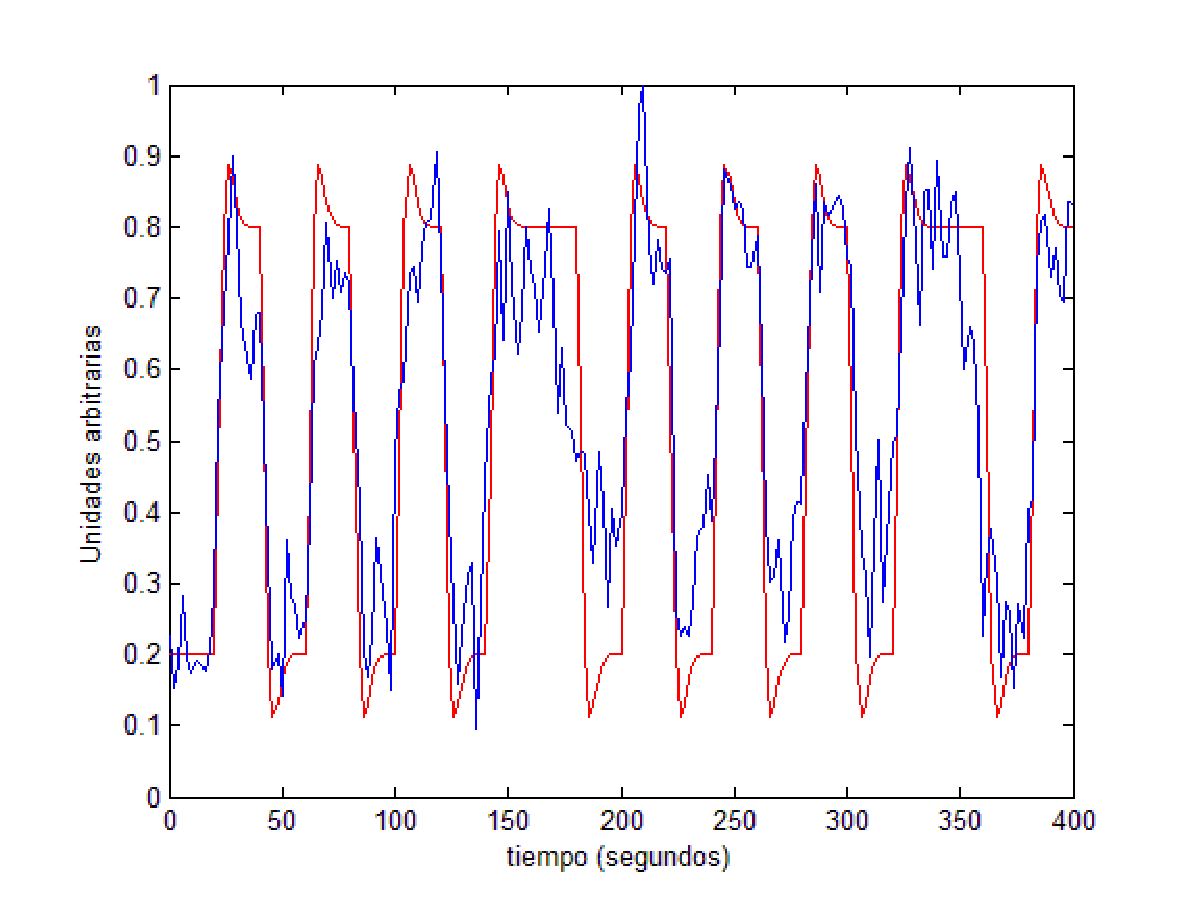
\includegraphics [width=0.7\textwidth]{glm_figura03.eps}
    \caption{Respuesta hemodinámica (azul) en un único voxel a lo largo del tiempo en un estudio de fMRI y su predicción mediante la convolución de una HRF doble gamma sobre el diseño de bloques (rojo).}
    \label{fig:glm03}
    \end{figg}
\end{figure}


Finalmente, en la figura \ref{fig:glm03} se ilustra la señal esperada al convolucionar la HRF sobre el diseño de los bloques. Se observa que el solapamiento sobre la señal BOLD observada es mejor que si sólo se tiene en cuenta el diseño de los bloques, el cual no asume el desfase inicial y el consecuente decaimiento de la respuesta hemodinámica (figura 1). El GLM toma la convolución del diseño de bloques como una variable predictora en la matriz de diseño ($X$), a modo de hacer una mejor predicción sobre la señal BOLD a lo largo de todos los \textit{voxels} ($Y$).


\section{Aplicación del Modelo Lineal General en un estudio de fMRI}

En este apartado se expone de manera simplificada un experimento de memoria de trabajo (N-back) en un estudio de fMRI para un solo participante\footnote{En el enlace \url{github.com/zchuri} se encuentra un tutorial para aplicar un GLM a datos de fMRI}. El paradigma N-back consiste en la presentación sucesiva de imágenes en este caso el participante tiene que recordar por bloques si la imagen presentada coincide con la anterior (1-back) o bien, con la presentada previa a la anterior (2-back). Por tanto, se va a modelar en base al GLM de modo que:

\begin{itemize}
  \item La variable dependiente ($Y$) será la señal BOLD para cada voxel a lo largo del tiempo.
  \item La matriz de diseño ($X$) constará de dos bloques uno para la tarea 1-back y otro para la tarea 2-back. Donde se convoluciona la presencia o ausencia de dicha tarea a lo largo del tiempo por una HRF de doble gamma.
  \item Los coeficientes para cada parámetro del modelo ($\beta$), es decir, habrá un coeficiente asociado a los bloques 1-back ($\beta_1$) y otro coeficiente asociado a los bloques 2-back ($\beta_2$).
  \item El error asociado al modelo ($\epsilon$), que para asumir que el modelo tiene un buen ajuste debe seguir una distribución normal con media cero.
\end{itemize}

En la figura \ref{fig:glm04} se muestra un esquema del modelo GLM dado los supuestos del experimento en cuestión.

\begin{figure}
	\begin{figg}
    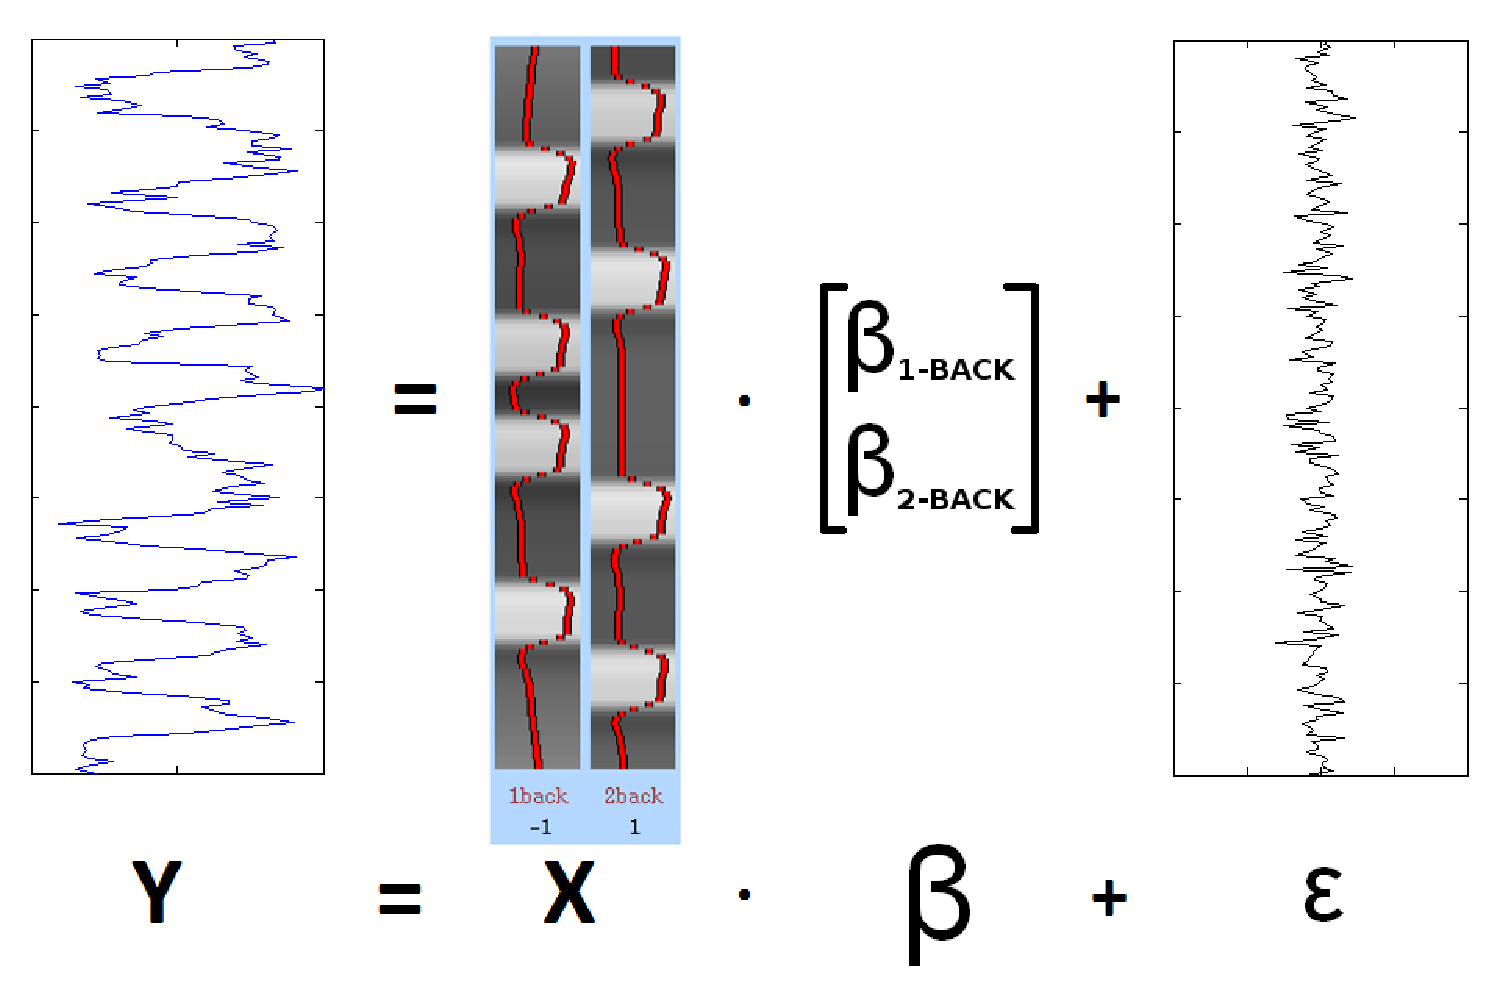
\includegraphics [width=0.7\textwidth]{glm_figura04.eps}
    \caption{Esquema del GLM, abajo, junto con su representación gráfica, arriba, en el experimento de fMRI de memoria de trabajo N-back.}
    \label{fig:glm04}
    \end{figg}
\end{figure}




Una vez que se ha aplicado dicho ajuste a todos los \textit{voxels} de interés el siguiente paso es realizar un análisis estadístico sobre qué tan bueno fue el ajuste. Es decir, se aplica un test estadístico sobre los coeficientes asociados a los parámetros, donde se asume que si el coeficiente es mayor el efecto de su bloque asociado en el ajuste del modelo es mayor. En este ejemplo se va a evaluar una hipótesis para todos los ajustes del modelo: si el coeficiente asociado a la tarea 2-back es mayor a la tarea 1-back. Dado que suponemos que la tarea 2-back es más demandante en términos de memoria de trabajo que la tarea 1-back. Dicha hipótesis sigue una distribución estadística, de modo que si el valor del estadístico resultante del contraste es bajo quiere decir que la diferencia entre ambos coeficientes no es significativamente diferente de cero, mientras que si el valor es suficientemente alto podemos asumir que hay una diferencia significativa entre los bloques y, por consiguiente, concluir que en tales \textit{voxels} su señal BOLD se ajustan al contraste de la hipótesis.

Otro aspecto relevante al considerar la significancia estadística de nuestro modelo sobre los datos observados es el control de los falsos positivos. El modelo va a aplicarse sobre un número ingente de \textit{voxels} (del orden de decenas de miles), por tanto, es necesario llevar a cabo una corrección de múltiples comparaciones. Algunos de los métodos más comunes en los datos de resonancia magnética son el \textit{random field theory}, \textit{false discovery rate} o test de permutaciones \cite{nichols2003controlling,lindquist2008statistical}.

Finalmente, es posible representar espacialmente aquellos \textit{voxels} donde la señal BOLD se ajusta significativamente a los contrastes mediante mapas estadísticos. En los resultados del estudio, se observa la significancia de los coeficientes del contraste en varios cortes axiales. A \textit{grosso modo}, se ve que hay un mejor ajuste del contraste 2-back $>$ 1-back en regiones de la corteza dorsal anterior y posterior, así como en la parte medial del lóbulo frontal (ver detalle en la Figura \ref{fig:glm05}). A las regiones significativas se les aplicó un método de múltiples comparaciones (\textit{family wise error}, o FWE, de \textit{random field theory}). Por tanto, podemos asumir que las regiones señaladas en el mapa estadístico son aquellas donde se recluta una mayor demanda hemodinámica ante tareas de memoria de trabajo tales como el N-back.



\begin{figure}
	\begin{figg}
    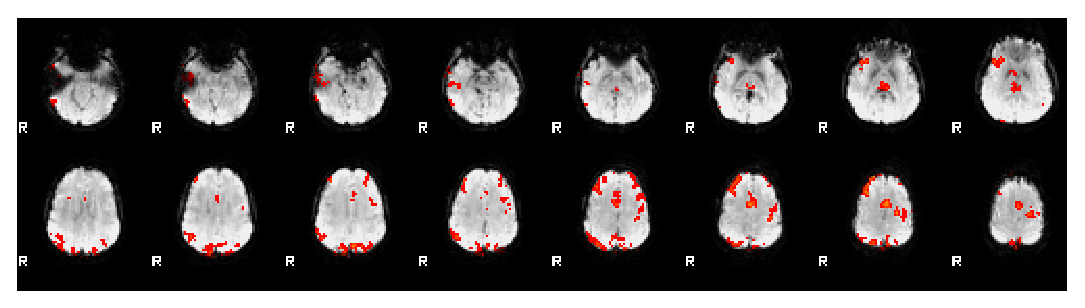
\includegraphics [width=0.7\textwidth]{glm_figura05.eps}
    \caption{Mapa de significancia del contraste 2-back $>$ 1-back, donde los valores significativos (p-valor < 0.05; FWE) aparecen en tonos rojo-amarillo. 'R' hace referencia al hemisferio derecho en cada uno de los cortes axiales.}
    \label{fig:glm05}
    \end{figg}
\end{figure}



\section{Conclusión}

De modo breve hemos repasado los parámetros del GLM, el cual sigue unos lineamientos bastante sencillos a pesar de que cuenta con suposiciones bastante rígidas, pero de todos modos, la gran ventaja del GLM es su versatilidad y flexibilidad, además de poseer un cómputo relativamente sencillo (\cite{lindquist2008statistical}).

El capítulo se centró básicamente a la aplicación del GLM en estudios de fMRI y de su consecuente señal BOLD, sin embargo, la aplicación del GLM no acaba aquí, también se puede aplicar a otras técnicas de neuroimagen y además, puede generalizarse al estudio de varios sujetos o varios grupos de interés.

Finalmente, podemos observar un ejemplo sencillo de aplicación del modelo conociendo el diseño de bloques y asumiendo como se va a comportar la respuesta hemodinámica. La gran mayoría de los paquetes que analizan datos de neuroimagen (e incluso cualquier otro tipo de datos) tienen implementados al menos una alternativa de generar el GLM, dado que a pesar de sus desventajas es una herramienta robusta y eficiente para evaluar hipótesis entre variables (\cite{monti2011statistical}).

%--------------------------------
%Bibliography
% \printbibliography

% \end{document}
